\begin{infocard}{Enlace iónico}
    Los \textbf{enlaces iónicos} se forman cuando un átomo pierde uno o más electrones y el otro átomo gana uno o más electrones.
    Ganar o perder electrones puede llenar la capa electrónica externa de un átomo y hacer que este sea energéticamente más estable, como se muestra en siguiente figura:

    \begin{figure}[H]
        \centering
        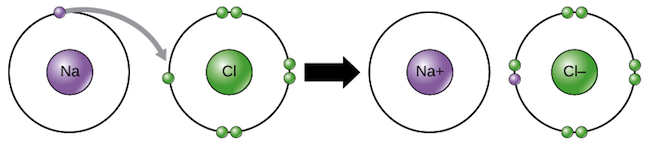
\includegraphics[width=\linewidth]{../images/a05bd453d0dc5add39892ed10f63bc92a5508539}
    \end{figure}
\end{infocard}